%% Section 3 - Propositional logic - calculus

\section{Lógica proposicional - cálculo proposicional}
%
\subsection{Tabela verdade}
%
\begin{frame}[t]
    \frametitle{Tabela verdade}
    \framesubtitle{True table of operators}
    %
    \begin{alertblock}{Definição}
        \small
        Segundo o princípio do \textbf{terceiro excluído}, toda proposição simples $p$ ou composta $H(p,q,...)$ só pode assumir \textbf{valor lógico} igual a \\ [1pt]
        \center{$V$ (verdade - \textit{TRUE}) \qquad ou \qquad  $F$ (falsidade - \textit{FALSE})} \\ [4pt]
        A \textbf{tabela-verdade} sintetiza o resultado de funções lógicas para $n$ proposições.
    \end{alertblock}
    %
    \vspace{-4mm}
    %
    \begin{figure}[c]
        \centering
        \caption{Tabela verdade para um estado(proposição) único.}
        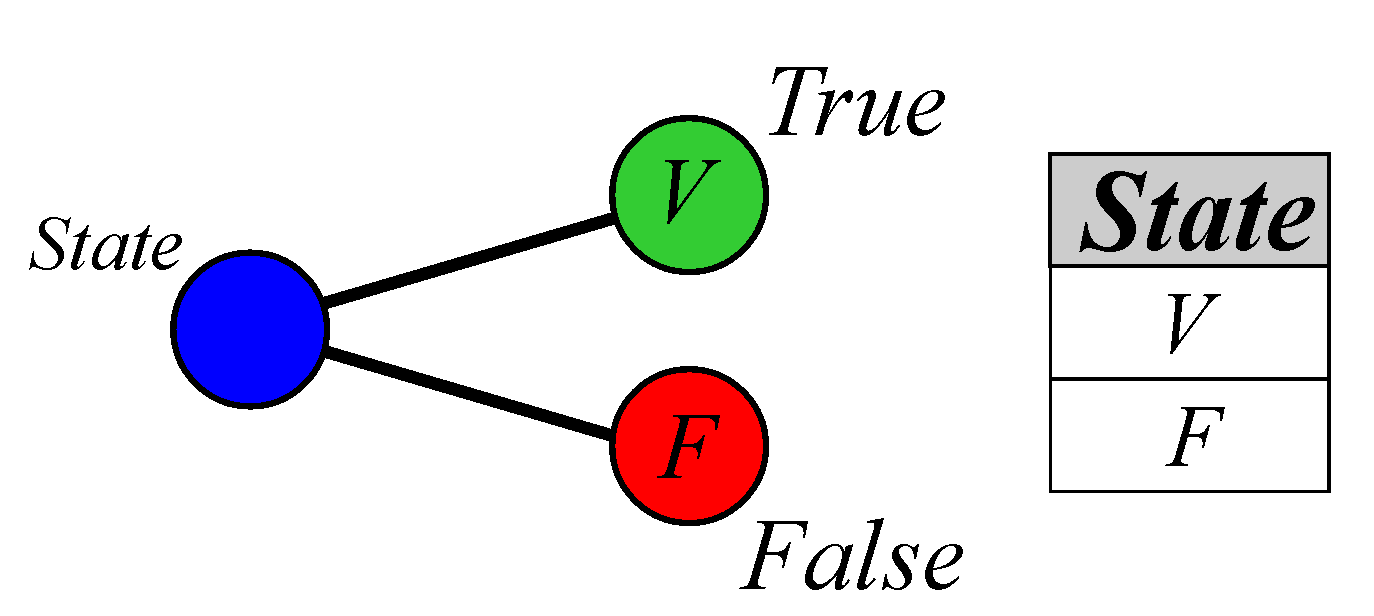
\includegraphics[scale=0.25]{TT2.png}
        \label{fig:tabela-verdade1}         
    \end{figure}
\end{frame}
%
\begin{frame}[c]
    \frametitle{Tabela verdade}
    \framesubtitle{Examples}
    %
    \begin{figure}[c]
        \centering
        \caption{Tabela verdade para uma proposição composta $H(p,q)$.}
        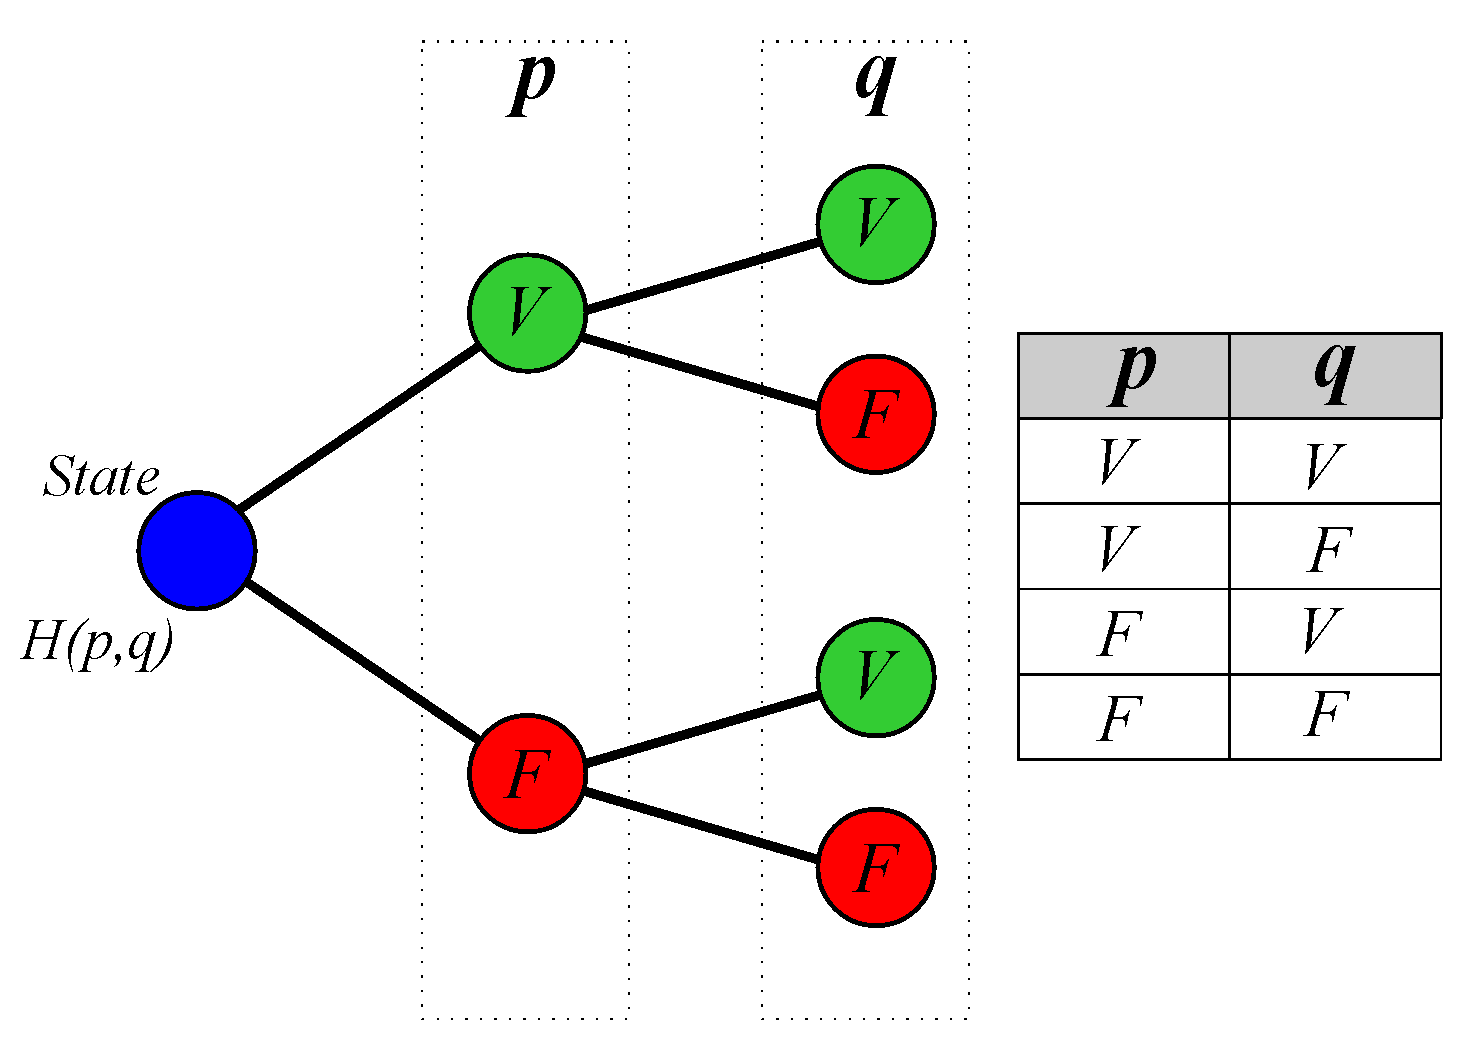
\includegraphics[scale=0.30]{TT3.png}
        \label{fig:tabela-verdade2}
    \end{figure}
\end{frame}
%
\begin{frame}[c]
    \frametitle{Tabela verdade}
    \framesubtitle{Examples}
    %
    \begin{figure}[c]
        \centering
        \caption{Tabela verdade para uma proposição composta $H(p,q,r)$.}
        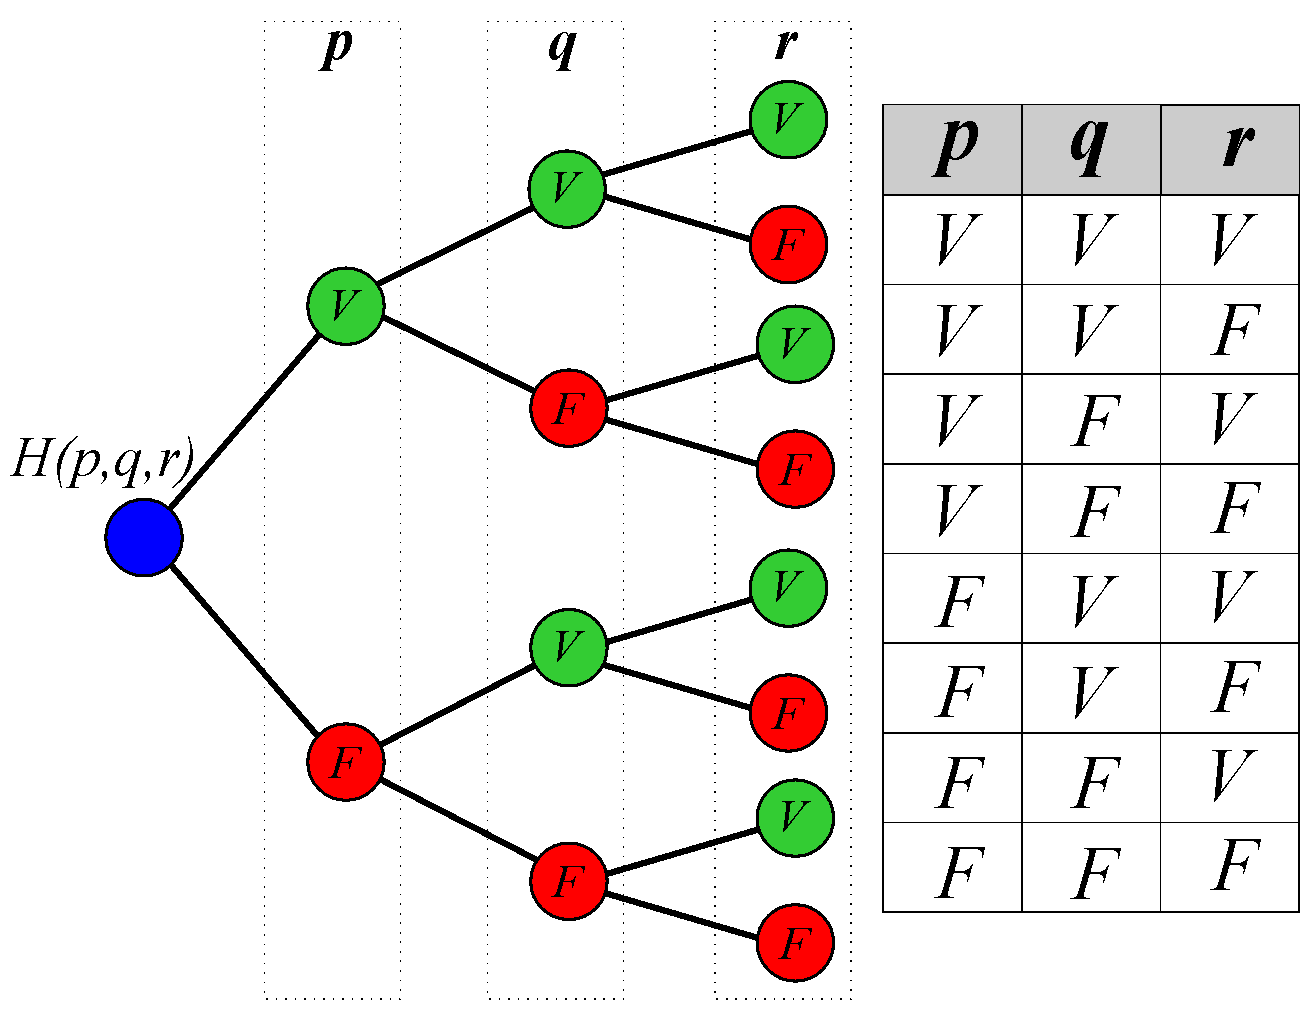
\includegraphics[scale=0.30]{TT4.png}
        \label{fig:tabela-verdade3}
    \end{figure}
\end{frame}
%
\subsection{Ordem de precedência e comprimento de fórmulas}
%
\begin{frame}[t]
    \frametitle{Definições complementares}
    \framesubtitle{Final considerations of the section - Procedence order}
    %
    \small
    \setbeamercolor{block title}{use=structure,fg=white,bg=black!75!black}
    \begin{block}{Ordem de precedência}
        \begin{itemize}
            \item Maior precedência: $\lnot$ ou $\sim$ 
            \item Precedência intermediária: $\rightarrow$ e $\leftrightarrow$
            \item Menor precedência: $\land$ e $\lor$
        \end{itemize}        
    \end{block}
    %
    \pause
    %
    \setbeamercolor{block title}{use=structure,fg=white,bg=orange!75!black}
    \begin{block}{Comprimento de uma fórmula}
        \begin{itemize}
            \item Se $H$ é um símbolo proposicional ou de verdade então $comp[H]=1$
            \item Se $H$ e $G$ são fórmulas da \textbf{lógica proposicional}, então
        \end{itemize}
        %\vspace{-3mm} % if negative it removes vertical space
        \begin{gather*}
            comp[\lnot H] = comp[H] + 1 \\
            comp[H \land G]~\text{ ou }~comp[H \lor G] = comp[H] + comp[G] + 1 \\
            comp[H \rightarrow G]~\text{ ou }~comp[H \leftrightarrow G] = comp[H] + comp[G] + 1
        \end{gather*}
        % gather environment: align equations on center
    \end{block}
\end{frame}
%
\subsection{Valor lógico}
%
\begin{frame}[t]
    \frametitle{Definições finais}
    \framesubtitle{Final considerations of the section 2/2}
    \small
    \begin{block}{Valor lógico}
        O \textbf{valor lógico} de uma proposição simples ou composta expressa seu valor resultante se \textit{verdadeiro} ou \textit{falso}.
        \begin{itemize}
            \item Para uma proposição simples $p$, $V(p)$ expressa seu valor lógico.
            \item Para uma proposição composta $H$, $V(H)$ expressa seu valor lógico.
        \end{itemize}
    \end{block}
        %
    \begin{columns}[T]
        \begin{column}{.5\textwidth}
            \begin{exampleblock}{Exemplo 1}
                \quad $p$ : O sol é verde. \\
                \quad $q$ : O sol é quente. \\
                \quad $r$ : O mar não é vermelho.\\[4pt]
                \quad $V(p) = V$, $V(q) = F$, $V(\lnot r)=F$ \\
                \quad $V(p \land q) = F$, \quad $V(q \lor r) = V$
            \end{exampleblock}
        \end{column}
        %
        %\hspace{5mm}
        \begin{column}{.5\textwidth}
            \begin{exampleblock}{Exemplo 2}
                \quad $p_1$ : $x \geq 10$   \\
                \quad $p_2$ : $x < 50$\\
                \quad $p_3$ : $x > 25$ \\[4pt]
                $V(p_1) = V$, $V(p_2) = F$, $V(\lnot p_3)=F$ \\
                \quad $V(p_1 \land p_2) = V$, $V(p_3 \land p_2) = F$
            \end{exampleblock}
        \end{column}
    \end{columns}
\end{frame}
%
\subsection{Exercícios}
%
\begin{frame}[t] % \renewcommand{\theenumi}{\alph{enumii}}
    \frametitle{Exercícios - 1/2}
    \framesubtitle{Practice the chapters concepts}
    %
    \small
    \setbeamercovered{invisible}
    \setbeamercolor{enumerate item}{fg=red!80!black}
    \setbeamertemplate{enumerate items}[default]
    \begin{exampleblock}{1. Identifique os itens abaixo que não são fórmulas da lógica proposicional.}
        \begin{columns}[T]
            \begin{column}{0.15\textwidth}
                \begin{enumerate}[\bf a.]
                    \item $pq$
                    \item $PQ$
                    \item $PQ \lnot$
                    \item $\lnot PQ$
                \end{enumerate}
            \end{column}
            %
            \hspace*{-5mm}
            %
            \begin{column}{0.15\textwidth}
                \begin{enumerate}[\bf a.]
                    \addtocounter{enumi}{4}
                    \item $p \land q$
                    \item $P \lor Q$
                    \item $PQ \land$
                    \item $\lor PQ$
                \end{enumerate}
            \end{column}
            %
            \hspace*{-5mm}
            %
            \begin{column}{0.20\textwidth}
                \begin{enumerate}[\bf a.]
                    \addtocounter{enumi}{8}
                    \item $p \rightarrow q$
                    \item $PQ \rightarrow$
                    \item $\rightarrow PQ \lnot$
                    \item $P \rightarrow Q \rightarrow $
                \end{enumerate}
            \end{column}
            %
            \hspace*{-7mm}
            %
            \begin{column}{0.2\textwidth}
                \begin{enumerate}[\bf a.]
                    \addtocounter{enumi}{12}
                    \item $P \rightarrow Q$
                    \item $P \leftrightarrow Q$
                    \item $P \leftrightarrow q$
                    \item $\leftrightarrow P \leftrightarrow Q$
                \end{enumerate}
            \end{column}
            %
            \hspace*{-8mm}
            %
            \begin{column}{0.25\textwidth}
                \begin{enumerate}[a.]
                    \addtocounter{enumi}{16}
                    \item $P \rightarrow true$
                    \item $P \land true$
                    \item $true~P \leftrightarrow q$
                    \item $false~PQ \land$
                \end{enumerate}
            \end{column}
        \end{columns}
    \end{exampleblock}
    %
    \pause
    \vspace{-2mm}
    %
    \begin{alertblock}{Respostas}
        a, b, c, d, g, h, j, k, l, p, q, s, t
    \end{alertblock}
    %
    \pause
    \vspace{-2mm}
    %
    % \setbeamercolor{enumerate item}{fg=red!80!black}
    % \setbeamertemplate{enumerate items}[default]
    \begin{exampleblock}{2. Determine o comprimento das fórmulas a seguir.}
        \begin{columns}[T]
            \begin{column}{0.8\textwidth}
                \begin{enumerate}[\bf a.]
                    \item $((\lnot \lnot~P \land Q) \leftrightarrow (P \rightarrow Q)) \land~true$
                    \item $(\lnot P \rightarrow (Q \lor R)) \leftrightarrow ((P \land Q) \leftrightarrow (\lnot \lnot R \lor \lnot P))$
                    \item $((P \lor Q) \rightarrow (P \rightarrow (\lnot Q)))$
                \end{enumerate}
            \end{column}
            %
            \pause
            %
            \begin{column}{0.2\textwidth}
                \begin{enumerate}[\bf a.]
                    \item 11
                    \item 17
                    \item 8
                \end{enumerate}
            \end{column}
        \end{columns}
    \end{exampleblock}
\end{frame}
%
\begin{frame}[t] % \renewcommand{\theenumi}{\alph{enumii}}
    \frametitle{Exercícios - 2/2}
    \framesubtitle{Practice the chapters concepts}
    %
    \small
    \setbeamercolor{enumerate item}{fg=red!80!black}
    \setbeamertemplate{enumerate items}[default]
    \begin{exampleblock}{3. Pesquise na internet as proposições para os problemas abaixo.}
        E, se possível, elabore a fórmula para avaliar um valor qualquer.\\
        \begin{enumerate}[\bf P1.]
            \item Verificar se um número $n \in \mathbb{Z} $ está no intervalo $\{n_1, n_2\}$ onde $n_1 < n_2$.
            \item Descobrir o maior entre 2 números.
            \item Descobrir o maior entre 3 números.
            \item Ordenar 2 números.
            \item Ordenar 3 números.
            \item Avaliar se um número é primo.
            \item Buscar letra em palavra (string).
            \item Transformar um tempo dado em \textbf{HH:mm:ss} em apenas \textbf{ss}.
        \end{enumerate}
    \end{exampleblock}
    %
    \normalsize
    \center{\textcolor{red}{\textbf{Trazer na próxima aula para tira-dúvidas.}}}
    \end{frame}